\begin{frame}{Blood Pressure Monitoring}
    \begin{columns}
        \column{0.5\columnwidth}
        \begin{itemize}

            \item Blood pressure
                  \begin{itemize}
                      \item Pressure against arterial wall
                      \item Systolic and diastolic pressures
                      \item mmHg
                  \end{itemize}


            \item Monitoring
                  \begin{itemize}
                      \item Intraoperative care
                      \item Hypotension \& Hypertension
                  \end{itemize}
        \end{itemize}

        \column{0.5\columnwidth}
        \begin{figure}
            \centering
            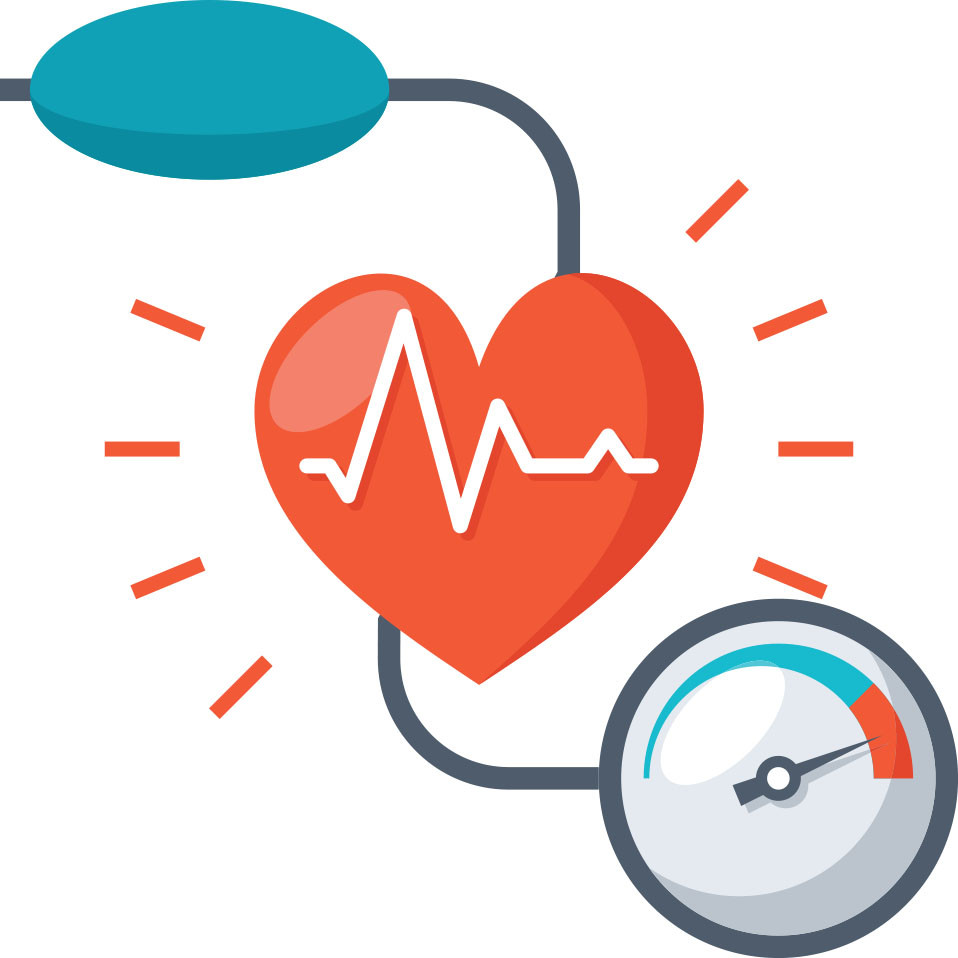
\includegraphics[width=0.5\columnwidth]{introduction/bp.jpg}
            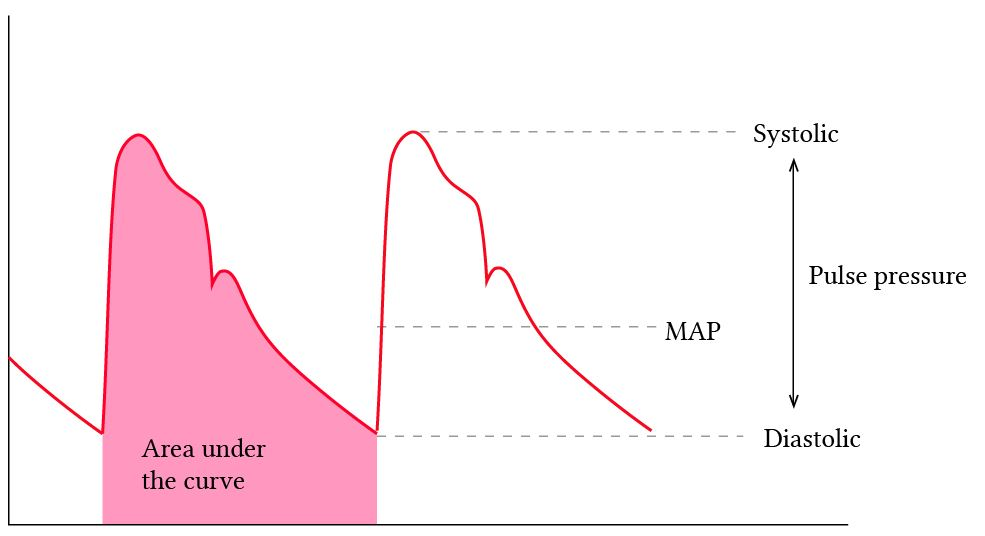
\includegraphics[width=\columnwidth]{introduction/systolicdiastolic.png}
        \end{figure}
    \end{columns}


\end{frame}

\begin{frame}{Context}{Application}
    \begin{columns}
        \column{0.5\columnwidth}
        \centering
        Clinical
        \begin{figure}
            \centering
            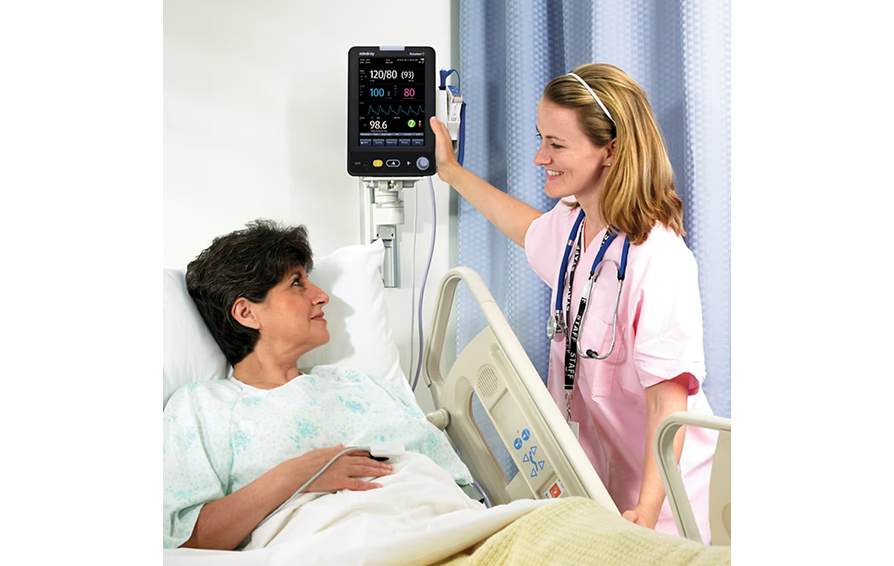
\includegraphics[width=\columnwidth]{introduction/clinical.png}
        \end{figure}

        \column{0.5\columnwidth}
        \centering
        EMS
        \begin{figure}
            \centering
            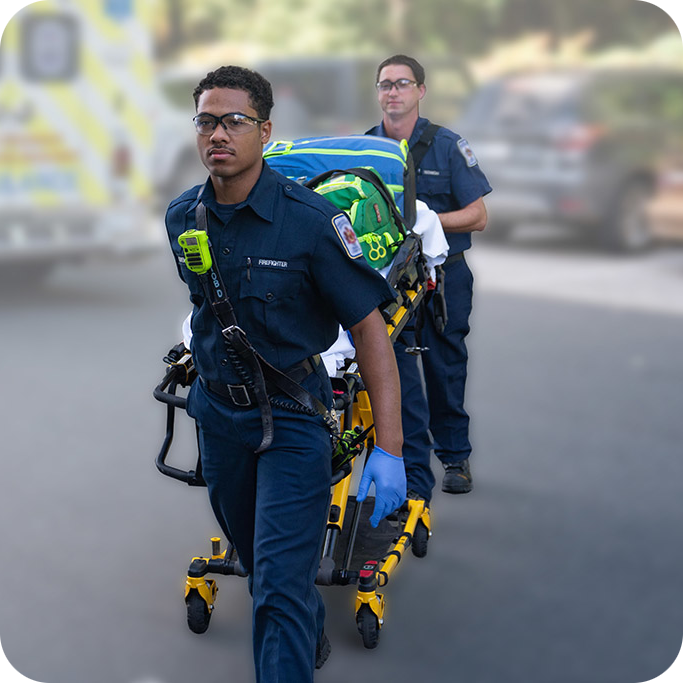
\includegraphics[width=\columnwidth]{introduction/ems.png}
        \end{figure}
    \end{columns}
\end{frame}

\begin{frame}{Context}{Sponsor}
    \begin{columns}
        \column{0.5\columnwidth}
        \begin{itemize}
            \item IMPACK CPR 
\includegraphics[height=2\fontcharht\font`\B]{introduction/impack.png}
            \item Chest Compression Device
            \item Feedback loop with vital signs
        \end{itemize}
        \begin{figure}
            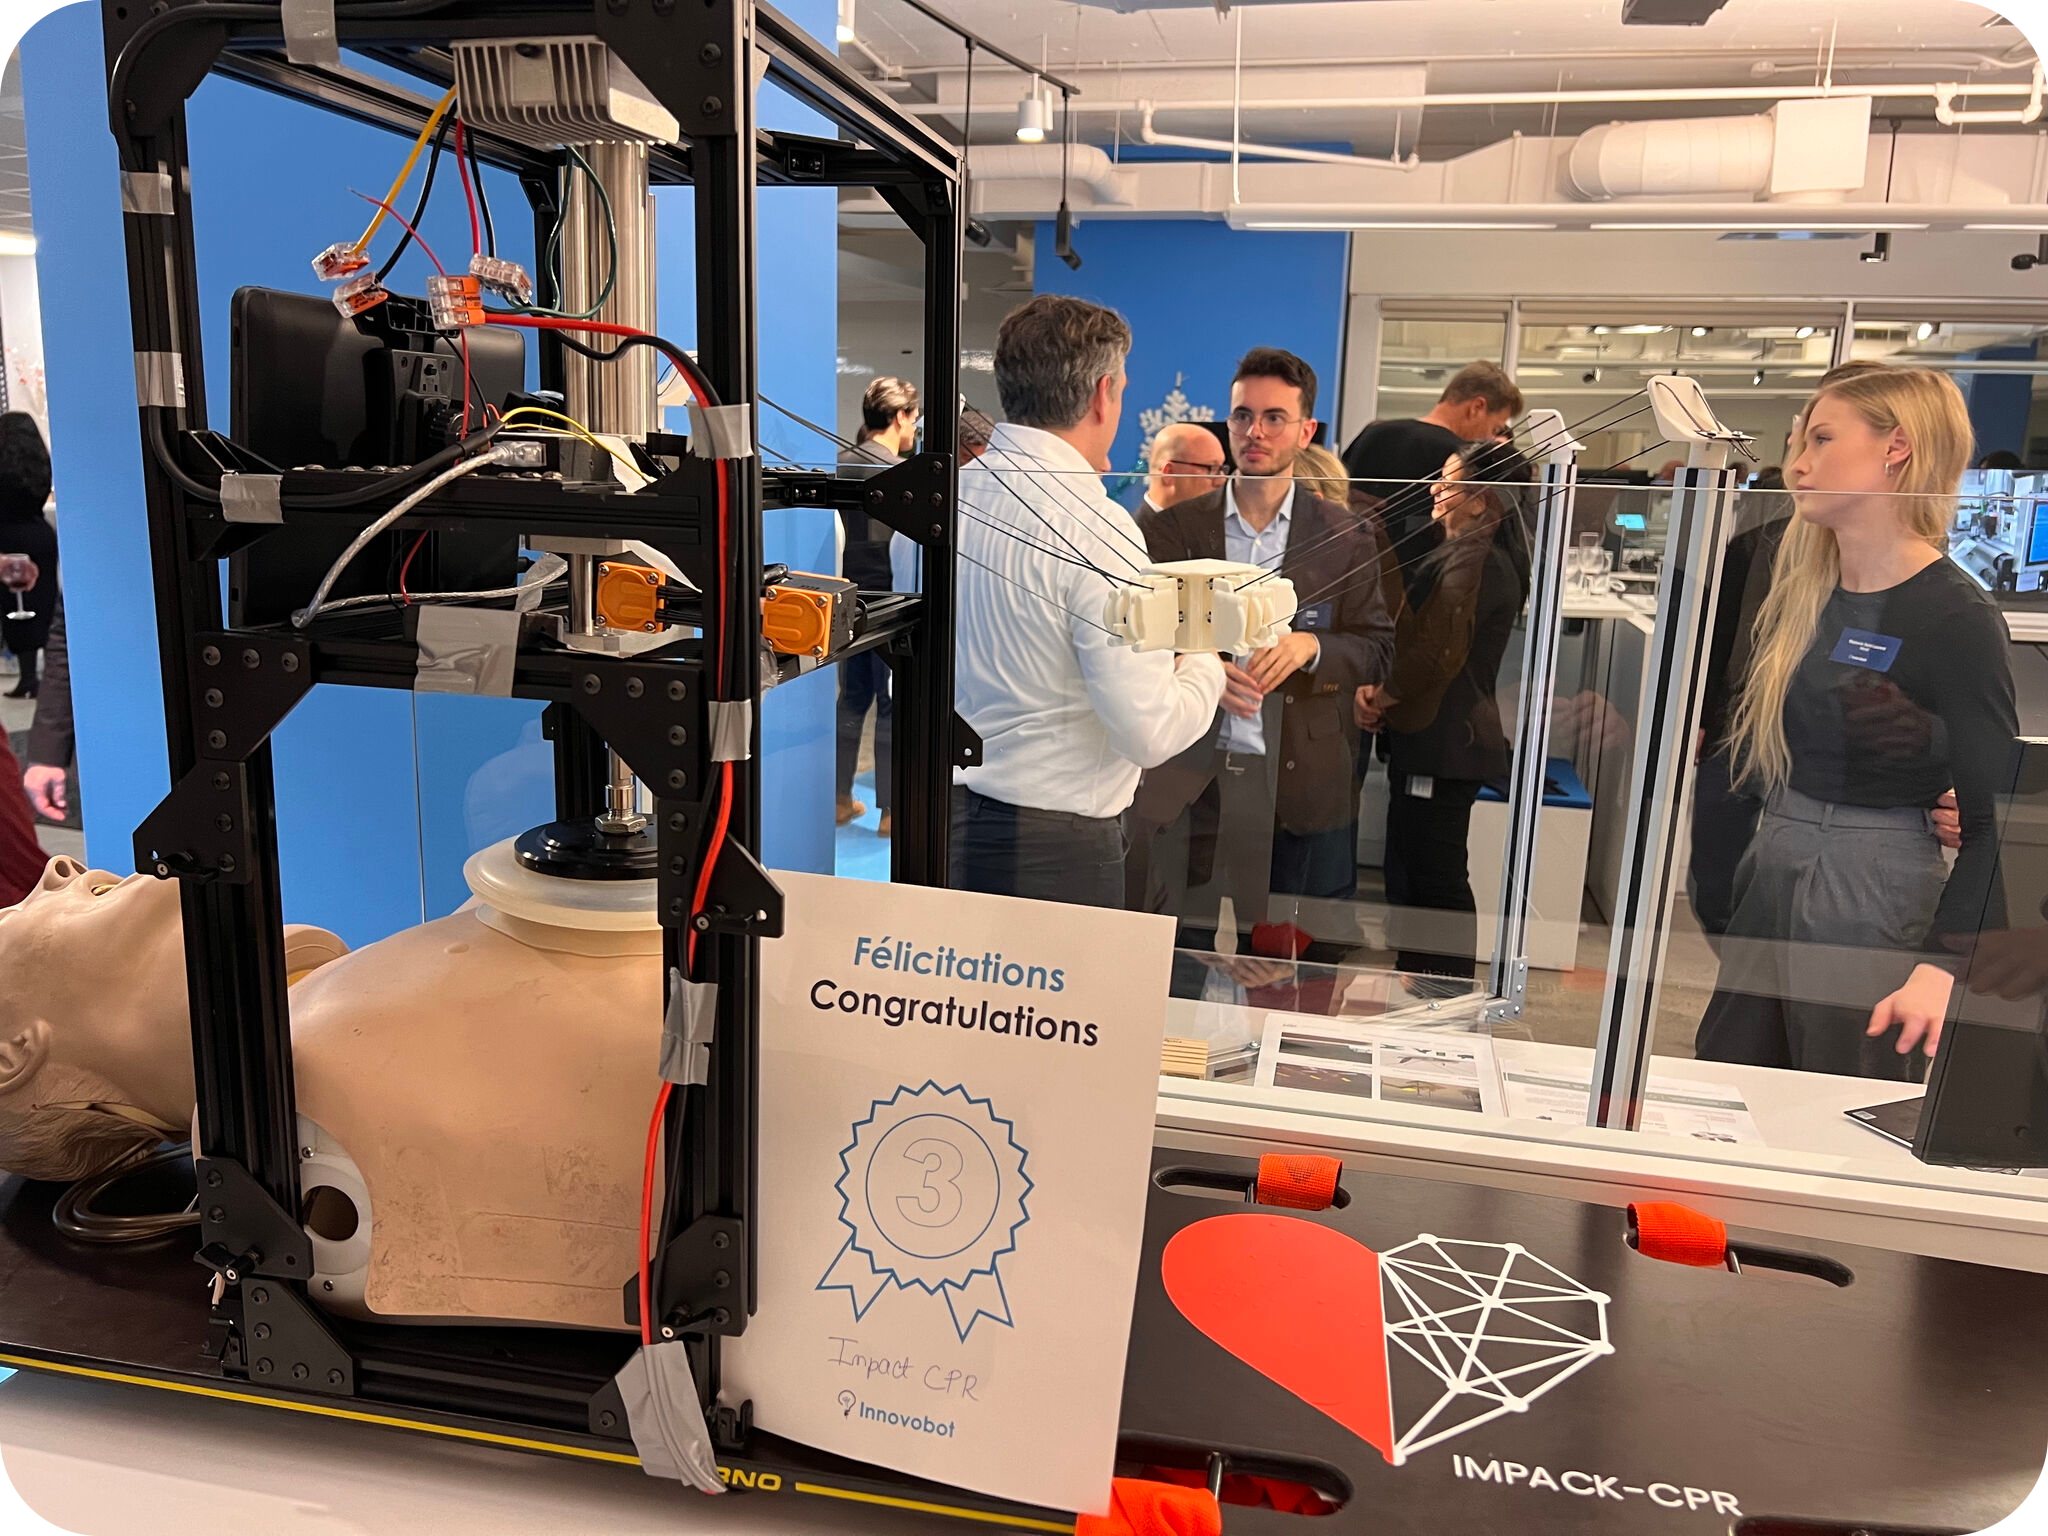
\includegraphics[width=\columnwidth]{introduction/masseur.png}
        \end{figure}

        \column{0.5\columnwidth}
        \begin{figure}
            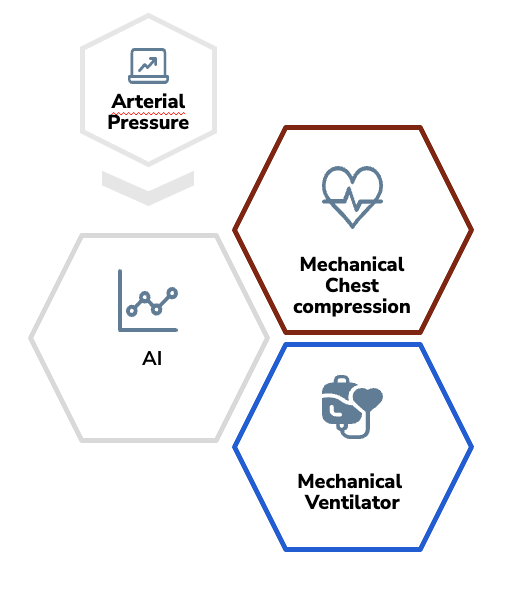
\includegraphics[width=\columnwidth]{introduction/loop.png}
        \end{figure}

    \end{columns}

\end{frame}

\begin{frame}{Current Solutions}
    \begin{columns}
        \column{0.5\columnwidth}
        \centering
        Cuff-based
        \begin{figure}
            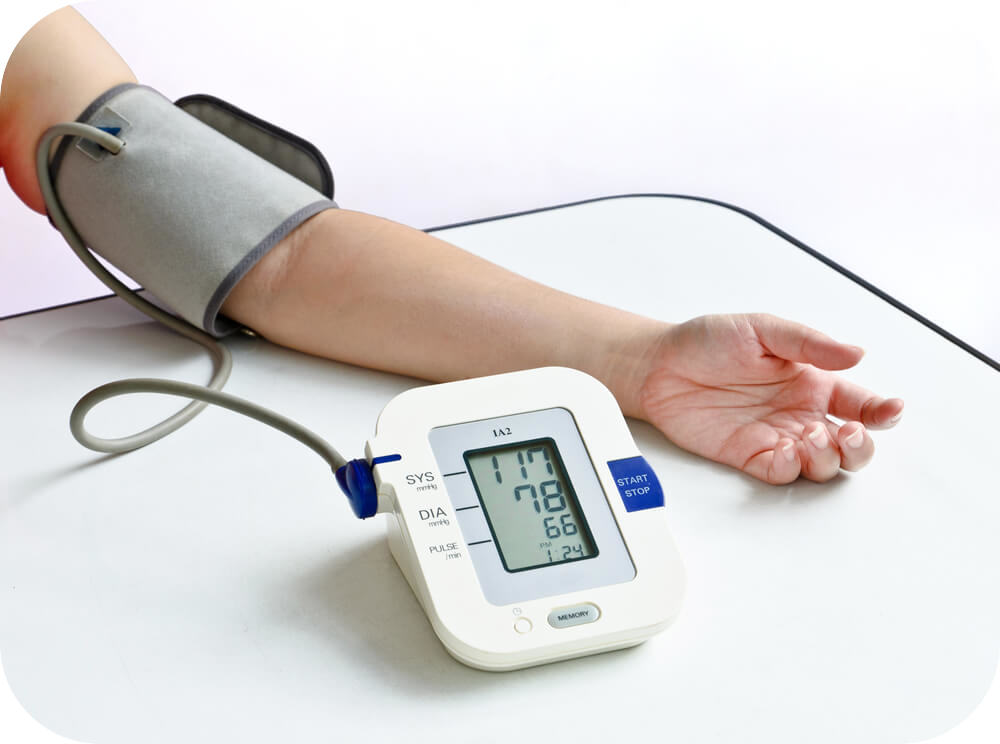
\includegraphics[width=\columnwidth]{introduction/cuff.png}
        \end{figure}
        % \begin{itemize}
        %     \item + non-invasive
        %     \item - not continuous
        % \end{itemize}

        \column{0.5\columnwidth}
        \centering
        Catheterization
        \begin{figure}
            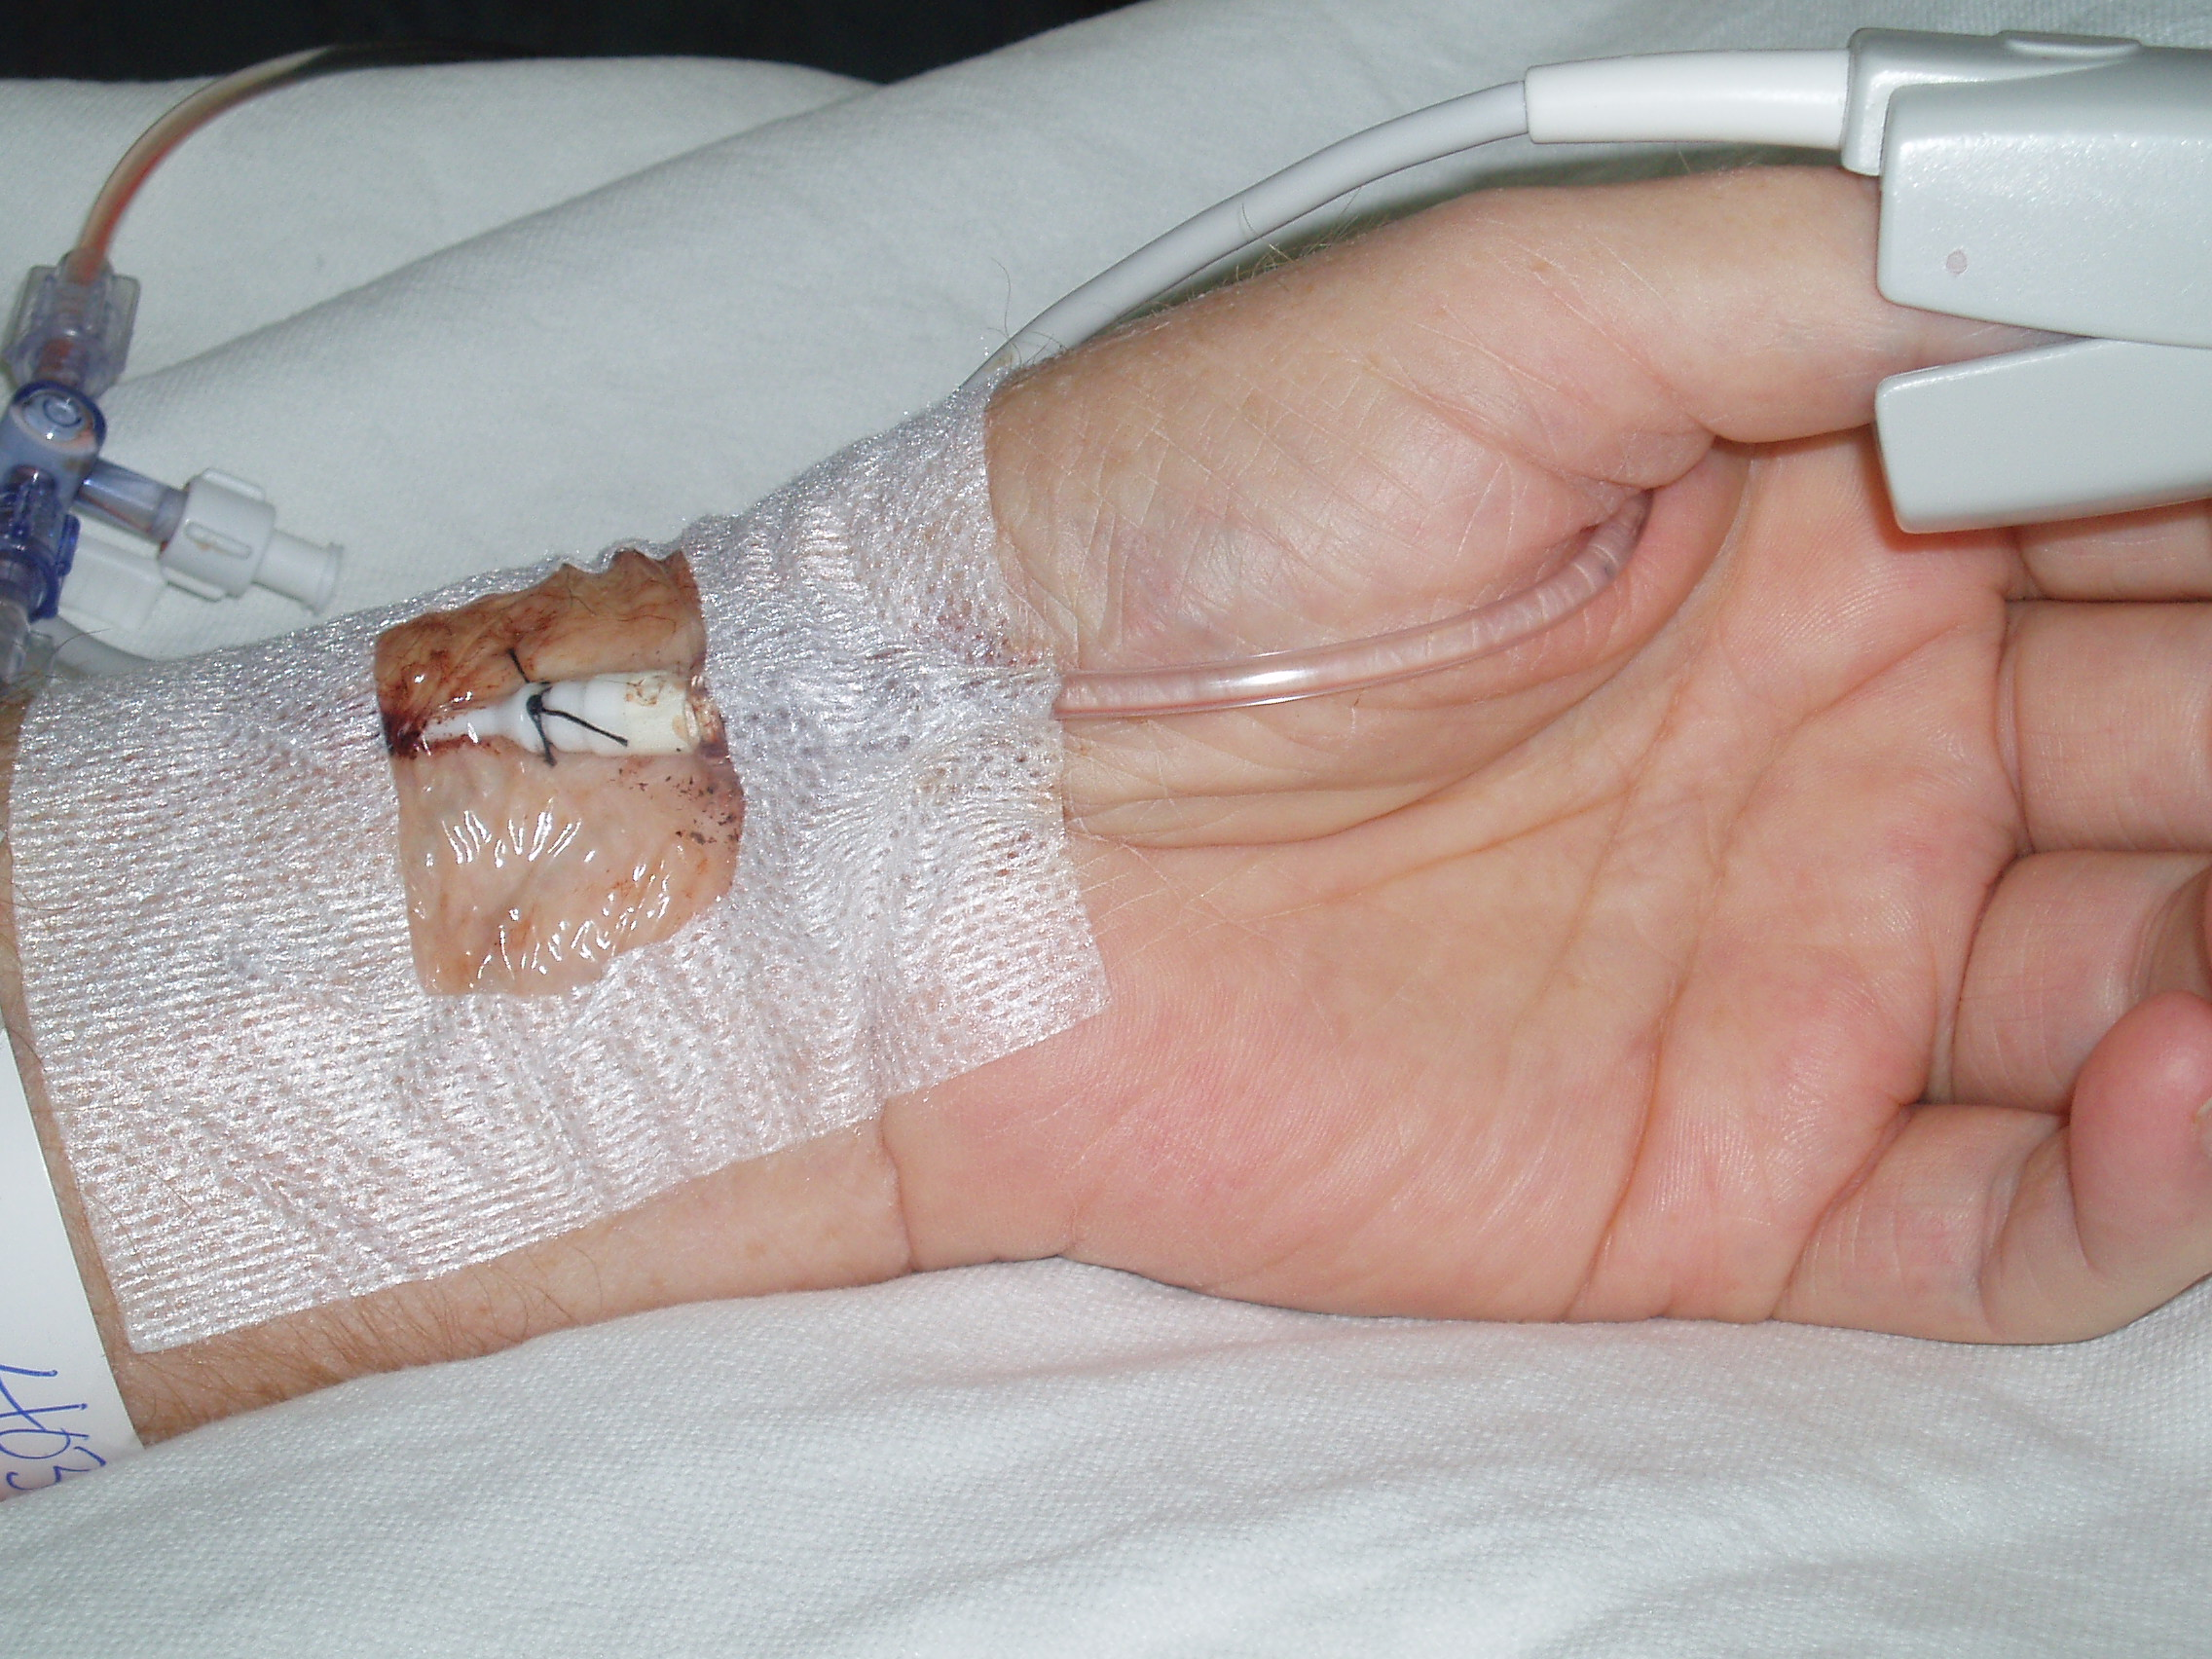
\includegraphics[width=\columnwidth]{introduction/catheter.png}
        \end{figure}
        % \begin{itemize}
        %     \item - invasive
        %     \item + continuous
        % \end{itemize}
    \end{columns}
    \begin{table}
        \begin{tabular}{r c c}
            \hline
                       & non-invasive & continuous \\
            \hline
            cuff-based & \cmark       & \xmark     \\
            catheter   & \xmark       & \cmark     \\
            \hline
        \end{tabular}
    \end{table}
\end{frame}

\begin{frame}{Goal}
    Properties of the desired system
    \begin{table}
        \begin{tabular}{r c c}
            \hline
                           & non-invasive & continuous \\
            \hline
            cuff-based     & \cmark       & \xmark     \\
            catheter       & \xmark       & \cmark     \\
            desired solution & \cmark       & \cmark     \\
            \hline
        \end{tabular}
    \end{table}
    Improve outcomes for patients
\end{frame}